\section{Ensemble Methods: Regression \& Multinomial Classification}
Ensemble methods can be applied widely, both in \textbf{regression} and \textbf{classification}. We have a slight focus of classification here.
\begin{itemize}
	\item Definition: \textbf{combination of multiple models}. Build and output different ''expert'' models, let them vote for decision. 
	\item Comparison over a \textbf{single model}: 
	\begin{itemize}
		\item a combination of several bad models sometimes achieves better result than a single good model. It ensembles different models with \textbf{low bias and high variance} and may
		\begin{itemize}
			\item reduce overall variance
			\item increase predictive performances
			\item decrease expected error (bias + variance)
		\end{itemize}
		\item ensemble models tend to be \textbf{more stable}, a small change in input data doesn't necessarily change the final prediction.
	\end{itemize}
	\item Types of Ensemble methods:
	\begin{itemize}
		\item Bagging
		\item Random Forest
		\item Boosting
		\item Stacking
	\end{itemize}  
\end{itemize}

\subsection{Bagging}
Bagging randomizes the \textbf{data} in training.
\begin{itemize}
	\item idea: reduces \textbf{variance} of \textbf{low-bias models}.
	\item Training Models (Training)
	\begin{itemize}
		\item randomly sample \textbf{m training subsets} of \textbf{size n} from the whole training data. (sample \textbf{with replacement}) 
		\item train one model for \textbf{each training subset independently} 
	\end{itemize}
	
	\item Classifying Instances (Testing)
	\begin{itemize}
		\item each trained model predicts the test data independently \textbf{with equal weight}.
		\item classification result: the \textbf{most frequent class}
	\end{itemize}
	\item Advantages:
	\begin{itemize}
		\item applied both in numeric prediction and classification
		\item works well when data is \textbf{noisy}
		\item improves performance if the learning scheme is \textbf{unstable} (eg: decision tree)
		\item can be \textbf{parallelized}.
	\end{itemize}
\end{itemize}
\subsection{Random Forest}
Random Forest \textbf{randomizes both data and feature selection}!!
\begin{itemize}
	\item Definition/Process: \textbf{aggregates} full grown trees with \textbf{low bias but high variance}. 
	
	$\rightarrow$ reduce the variance of the final predictor by \textbf{aggregating} all trees.
	\item Training Models:
	\begin{itemize}
		\item define the $n$ number of trees, and the $m$ number of attributes to try.
		\item for each tree, draw a \textbf{bootstrap sample of data} (random sample with replacement), \textbf{randomly select $m$ attributes}.
		\item train each tree with their selected attributes \textbf{independently}.
	\end{itemize}

	\item Classifying Instances:
	\begin{itemize}
		\item each trained model predicts the test data independently (default: with equal weight). 
		\item classification result: aggregate the tree, result is the \textbf{most frequent class}.
		\item \textbf{Weighting possible}. 
	\end{itemize}

\end{itemize}

\subsection{Boosting}
\begin{itemize}
	\item Idea: combines \textbf{weak learners} into a \textbf{strong learner}. 
	
	$\rightarrow$ reduces \textbf{bias} of \textbf{low-variance models}.
	\item Training Models (example: Adaboost):
	\begin{itemize}
		\item Initialization: all training instances have \textbf{equal weight}.
		\item First model:  is trained and predicts \textbf{the training data instances} back.
		\item Evaluation of prediction: \textbf{correct} prediction gets \textbf{lower} weights, \textbf{false} prediction gets \textbf{higher} weights.
		\item \textbf{based on the last model}, repeat step 2-3. Until $m$ models are trained, always focus on traing data \textbf{with high weights} -- misclassified instances. 
	\end{itemize}
	\item Classifying Instances: 
	\begin{itemize}
		\item each model is assigned \textbf{weight according to error rate} from training.
		\item each trained model predicts the test data independently.
		\item classification result: \textbf{weighted average} of classes.
	\end{itemize}
	\item Algorithms: AdaBoost(weighting instances), XGBoost(trained on residual errors), etc.
\end{itemize}

\subsection{Bagging VS. Boosting}
\begin{figure}[H]
	\centering
	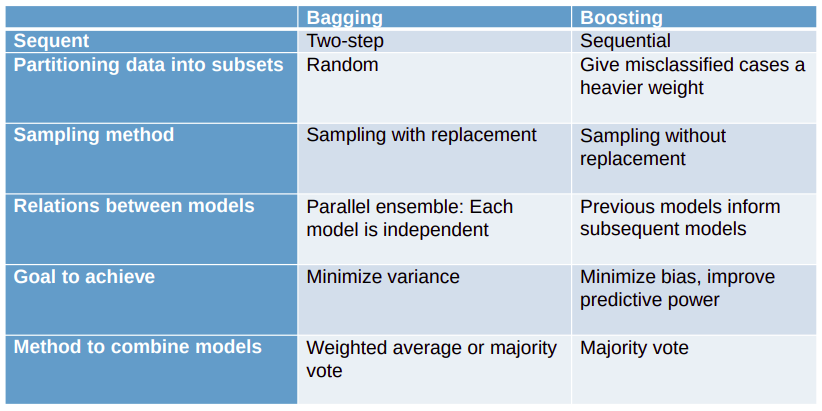
\includegraphics[width=0.85\textwidth]{bagging-boosting.png}
\end{figure}
\subsection{Stacking \& Meta-Learning}
\begin{itemize}
	\item Idea: different level models will be stacked on, predictions from \textbf{different classifiers(level-0 models)} are used as input into a \textbf{meta-learner(level-1 model)}. 
	\item Training Models -- level 0:
	\begin{itemize}
		\item split the training data into \textbf{training subset} and \textbf{holdout subset}.
		\item $m$ different models(NB, DT, etc.) are trained \textbf{independently} on the training subset. 
		
		$\rightarrow$ level-0 classifiers
	\end{itemize}
	\item Classifying Instances -- level 0:
	\begin{itemize}
		\item the level-0 classifiers predicts on \textbf{holdout subset}
		\item the holdout set contains \textbf{only the prediction results of all level-0 classifiers}.
	\end{itemize}
	\item Training Models -- level 1:
	\begin{itemize}
		\item training holdout serves as \textbf{training data} for a \textbf{single} level-1 model (normally simple, eg:regression).
	\end{itemize}
	\item Classifying Instances -- level 1:
	\begin{itemize}
		\item classify the test data with the level-1 model.
	\end{itemize}
\end{itemize}